\section{Problemstellung}

Die Kernidee hinter der Blockchain-Technologie ist es einen Intermediär zu substituieren, der nur eingesetzt wurde um eine neutrale Vertrauensbildung zu ermöglichen. \ac{dlt} verfolgt dabei den Ansatz die Vertrauensbildung, den Ablauf von Transaktionen und deren sichere Festschreibung mit mathematischen und kryptographischen Methoden zu realisieren. Im Kontrast zum konventionellen Intermediär, welcher durch eine dritte Person oder Institution wie z.B. eine Bank oder einen Notar repräsentiert wird.\\

Für das Problem der Einigkeit über den Zustand eines Werts innerhalb der Blockchain sind zwei generelle Verfahren etabliert. Die \ac{pow} und \ac{pos} genannten Algorithmen nutzen unterschiedliche Ansätze um Konsens innerhalb eines Netzwerks zu bilden und so Vertrauen herzustellen. Beide Verfahren haben ihre Vor- und Nachteile.\\

Die Energiebranche befindet sich seit Jahren im Umbruch. Alte Infrastrukturen, neue Technologien und Wettbewerbsanforderungen lassen sich zum aktuellen Zeitpunkt nicht wirklich effizient in einem System zusammenfassen. Der Energiemarkt wird immer fragmentierter durch kleine Stromerzeuger und neue Möglichkeiten der Stromerzeugung. In diesem Bereich existiert viel Optimierungspotential, das durch neue Technologien genutzt werden kann. Beispielsweise im Stromhandel zwischen Betreibern und Verbrauchern.\\

Prozesse die einen transaktionalen Charakter besitzen und oft auch ein oder mehrere Vermittlerstellen zwischengeschaltet haben würden sich Ideal für den Einsatz von Blockchain Technologie eignen. Fehlende Standards und generelle Unsicherheit verhindern allerdings den flächendeckenden Einsatz der Technologie.\\

Abbildung \ref{fig:statista-huerden-blockchain-2016} zeigt die Ergebnisse einer Umfrage des Fachmagazins Cofinpro zum Thema \glqq Wo sehen Sie Hürden für die Blockchain-Technologie?\grqq~. So scheinen die mit Abstand größten Einstiegsbarrieren fehlende Standards und rechtliche Regelungen zu sein.

\begin{figure}[h!]
	\centering
	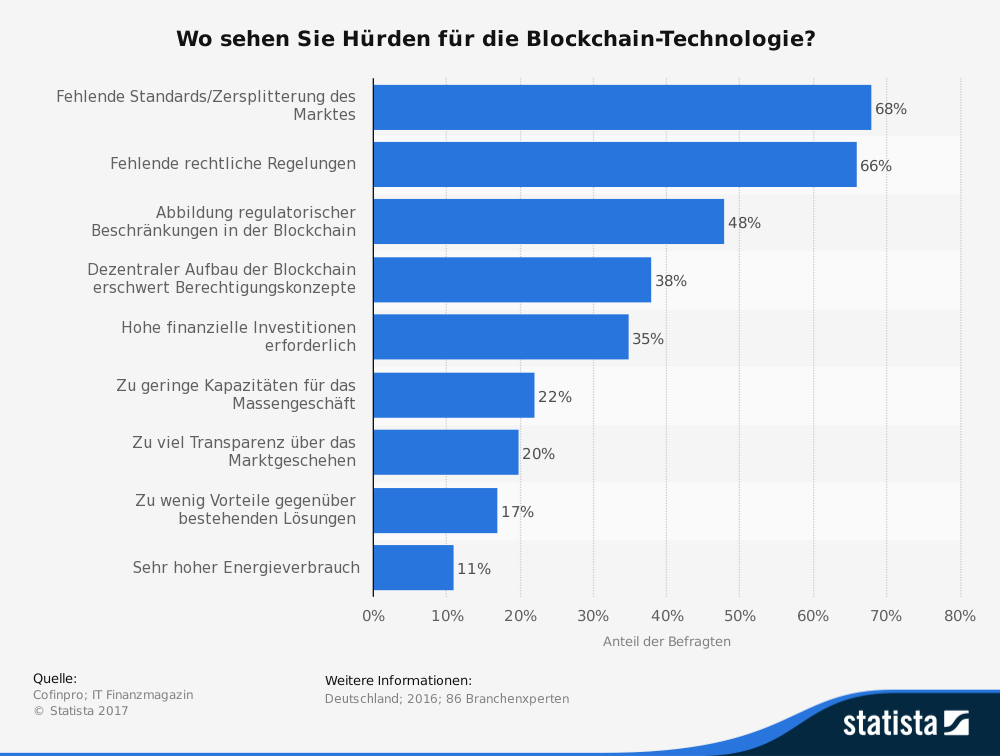
\includegraphics[width=0.7\linewidth]{pictures/Statista-Huerden-Blockchain-2016}
	\caption[Statista Blockchain Umfrage]{Cofinpro - Wo sehen Sie Hürden für die Blockchain Technologie? \cite{Cofinpro}}
	\label{fig:statista-huerden-blockchain-2016}
\end{figure}

Der technische Hintergrund einer Blockchain ist nicht neu. Die einzelnen Komponenten sind bereits heute vielfach erprobt im produktiven Einsatz. \cite{Diffie1976}\cite{Steinmetz2005} Die Kombination zu einer Blockchain ist allerdings neu und aktuell nur in Pilotprojekten für vereinzelte Use-cases zu finden.\\

Die \ac{dena} hat zusammen mit der privaten Hochschule ESMT Berlin von Führungskräften der deutschen Energiewirtschaft einschätzen lassen welche Bereiche und wie groß die Potentiale durch Blockchain-Technologie jeweils sind. Abbildung \ref{fig:dena-blockchain-use-cases} zeigt schematisch das Ergebnis, wobei eine dunklere Färbung eine höhere Übereinstimmung zwischen Herausforderung und Lösungsansatz mit Blockchain und die Größe der Kreise die Wahrscheinlichkeit für einen Einsatz in naher Zukunft zeigen. Der Umfrage ist zu entnehmen, dass über die Hälfte der Teilnehmer eine weitere Verbreitung von Blockchain Technologie in der Energiewirtschaft für wahrscheinlich halten. \cite[vgl.]{EnergieAgentur2016}\\

\begin{figure}[h!]
	\centering
	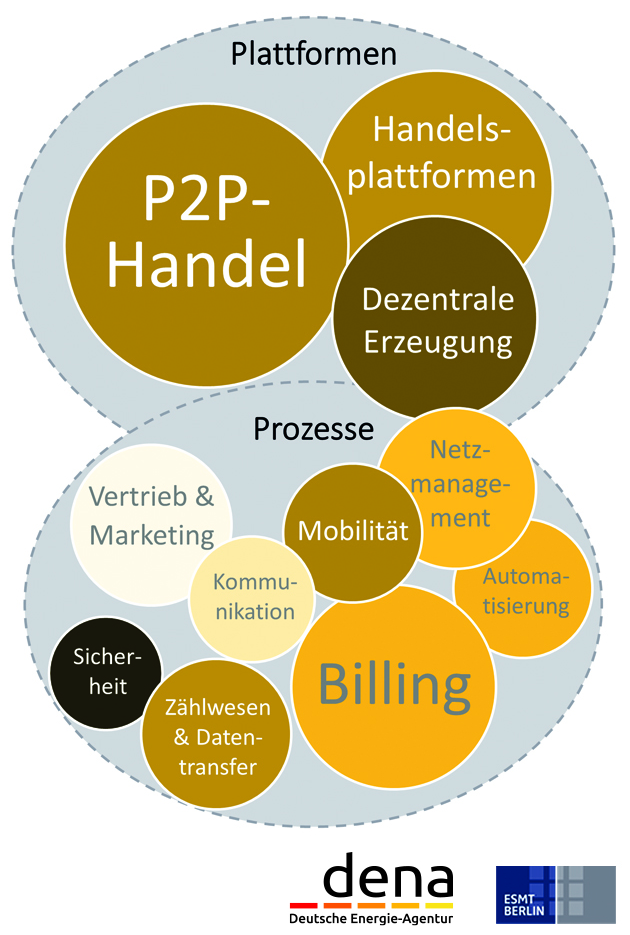
\includegraphics[width=0.8\linewidth]{pictures/dena-blockchain-use-cases}
	\caption[dena Potentielle Anwendungsfelder der Blockchain]{Potenzielle Anwendungsfelder der Blockchain \cite{EnergieAgentur2016}}
	\label{fig:dena-blockchain-use-cases}
\end{figure}

%Soll die Blockchain Technologie zum Einsatz kommen gibt es offene Fragen. Eine Blockchain ist keine Silberkugel für sämtliche betriebswirtschaftliche Prozesse. Viel mehr kann eine Blockchain als Skalpell dienen um präzise ein bestimmtes Problem zu lösen.\\

%\begin{itemize}
%	\item Technologie ist so neu und frisch verfügbar im Industriekontext
%	\item Ermittlung und Definition möglicher Geschäftsprozesse der Energiewirtschaft
%	\item Vorhandene Lösungen am Markt vergleichen für den Einsatz
%	\item Mehrwert eines DLT-basierten Geschäftsprozesses herausarbeiten
%	\item Spieltheorie neue Geschäftsfelder Blockchain
%\end{itemize}

%Video [Wir und die Blockchain (The Blockchain and Us) (2017) - Deutsche Synchronfassung/German version - YouTube](\url{https://www.youtube.com/watch?v=x2mKDWsNijo})

% konkrete Beschreibung des Problems

\newpage